\begin{frame}[fragile]{7-Segment Anzeigen}
	\metroset{block=fill}
	\begin{block}{Können Zahlen zeigen}
		\begin{center}
			\sevensegnum[size=15mm]{2}%
			\hspace{1em}
			\sevensegnum[size=15mm]{0}%
			\hspace{1em}
			\sevensegnum[size=15mm]{2}%
			\hspace{1em}
			\sevensegnum[size=15mm]{5}%
		\end{center}
	\end{block}
	\pause
	\begin{block}{Zeigen manchmal wirres Zeugs}
		\begin{center}
			\sevenseg[size=15mm]{0,0,0,1,0,0,0,}%
			\hspace{1em}
			\sevenseg[size=15mm]{0,1,0,0,1,0,0,}%
			\hspace{1em}
			\sevenseg[size=15mm]{1,1,0,1,1,1,1,}%
			\hspace{1em}
			\sevenseg[size=15mm]{1,0,1,1,0,0,0,}%
		\end{center}
	\end{block}
\end{frame}

\begin{frame}{\only<2->{\xout}{Der Checker} \only<2->{Das Prädikat}}
	Wir brauchen einen \textit{Checker}:
	\Huge
	\begin{center}
		$
			\only<1,2>{P_{\text{Zahl}}\left(\sevensegnum{6}\right)}
			\only<3->{P_{\text{Zahl}}\left(\sevenseg{{1,0,1,1,0,0,0,}}\right)}
		$
	\end{center}
	\normalsize
	% todo
	\only<1>{Wenn wir in diesen \textit{Checker} (genannt Prädikat) eine Anzeige einsetzen, haben wir eine logische Aussage}
	\only<2-3>{
		\begin{tikzpicture}[overlay]
			\node[] at (5,.8) (base) {};
			\node[] at (2, -.4) (wahr) {
				\only<2>{\alert}{Wahr}, wenn eine Zahl zu sehen ist
			};
			\draw[->] (base) to (wahr);
			\only<3>{\node[] at (8, -.4) (wahr) {
					\alert{Falsch}, wenn keine Zahl zu sehen ist
				};
				\draw[->] (base) to (wahr);
			}
		\end{tikzpicture}
	}
\end{frame}

{\setbeamercolor{palette primary}{bg=ExColor}
\begin{frame}{Denkpause}
	Sind die folgenden Aussagen wahr oder falsch
	\metroset{block=fill}
	\begin{block}{Normal}
		\begin{itemize}
			\item $A_1$: $P_{\text{Zahl}}\left(\sevensegnum[]{7}\right)$ \only<2->{\hspace{1cm}wahr}
			\item $A_2$: $P_{\text{Zahl}}\left(\sevenseg[]{0,1,0,0,1,0,1}\right)$ \only<3->{\hspace{1cm}falsch}
			\item $A_3$: $P_{\text{Zahl}}\left(\sevensegnum[]{4}\right)$ \only<4->{\hspace{1cm}wahr}
			\item $A_4$: $P_{\text{Zahl}}\left(\sevenseg[]{1,0,1,0,1,0,1}\right)$ \only<5>{\hspace{1cm}falsch}
		\end{itemize}
	\end{block}
\end{frame}
}

\begin{frame}{Zurück zu unserem Beispiel}
	Wie reparieren wir die Anzeige?
	\begin{center}
		\sevenseg[size=15mm]{0,0,0,1,0,0,0,}
		\hspace{1em}
		\sevenseg[size=15mm]{0,1,0,0,1,0,0,}
		\hspace{1em}
		\sevenseg[size=15mm]{1,1,0,1,1,1,1,}
		\hspace{1em}
		\sevenseg[size=15mm]{1,0,1,1,0,0,0,}
	\end{center}
\end{frame}

\begin{frame}{Funktionen}
	Wir brauchen eine Funktion, die Segmente einschaltet
	\Large
	\begin{center}
		$
			f_{\text{On}}\left(
			\sevenseg[size=10mm]{1,0,0,1,0,0,1,},
			\sevenseg[size=10mm]{0,1,1,0,1,1,0,}
			\right) =
			\sevenseg[size=10mm]{1,1,1,1,1,1,1,}
		$
	\end{center}
\end{frame}


\begin{frame}{Reicht das?}
	\begin{itemize}
		\item<1-> $f_{\text{On}}\left(\sevenseg{{0,0,0,1,0,0,0,}}, \only<1>{\hspace{1em}}\only{\sevenseg{{1,1,0,0,1,0,1,}}}<2->\right) = \sevensegnum{2}$
		\item<3-> $f_{\text{On}}\left(\sevenseg{{0,1,0,0,1,0,0,}}, \only<3>{\hspace{1em}}\only{\sevenseg{{1,0,1,1,0,1,0,}}}<4->\right) = \sevensegnum{0}$
		\item<5-> $f_{\text{On}}\left(\sevenseg{{1,1,0,1,1,1,1,}}, \only<5>{\hspace{1em}}\only{\textcolor{red}{X }}<6->\right) = \sevensegnum{2}$
		\item<7-> $f_{\text{On}}\left(\sevenseg{{1,0,1,1,0,0,0,}}, \only<7>{\hspace{1em}}\only{\sevenseg{{0,0,0,0,0,1,1,}}}<8->\right) = \sevensegnum{5}$
	\end{itemize}
\end{frame}


\begin{frame}{Mehr Funktionen}
	\Large
	\begin{center}
		$
			f_{\text{Off}}\left(
			\sevenseg[size=10mm]{{1,1,1,1,1,1,1,}},
			\sevenseg[size=10mm]{{0,1,1,1,1,1,0,}}
			\right) =
			\sevenseg[size=10mm]{{1,0,0,0,0,0,1,}}
		$
	\end{center}
	\normalsize
\end{frame}

\begin{frame}{Mehr Funktionen}
	\Large
	\begin{center}
		$
			f_{\text{Off}}\left(
			\sevenseg[size=10mm]{1,1,1,1,1,1,1,},
			\sevenseg[size=10mm]{1,1,1,1,1,1,0,}
			\right) =
			\sevenseg[size=10mm]{0,0,0,0,0,0,1,}
		$
	\end{center}
	\normalsize
\end{frame}


\begin{frame}{Beides Zusammen}
	Kombiniert mit unserem \alert{Prädikt}:
	\Large
	\begin{center}
		$
			P_{\text{Zahl}}\left(f_{\text{On}}\left(
			\sevenseg[size=10mm]{1,0,0,0,0,0,0,},
			\sevenseg[size=10mm]{0,1,1,0,0,0,0,}
			\right)\right)
		$
	\end{center}
	\normalsize
	\pause
	Diese Aussage ist wahr
	\par
	\pause
	Allgemeiner:
	$U =\left\{\sevensegnum[]{0},\sevenseg{{0,1,1,0,1,1,1,}},\sevensegnum[]{2},\sevenseg{{0,1,1,0,0,0,0,}},\sevensegnum[]{4},\sevenseg{{0,0,0,0,0,0,0,}},\sevenseg{{0,1,1,1,1,1,0,}},\sevensegnum[]{7},\sevensegnum[]{8},\sevenseg{{0,0,1,0,1,1,1,}}, \dots \right\}$
	$$
		\forall X\in U:\exists Y \in U: P_{Zahl}(f_{On}(X,Y))
	$$
	$U =\left\{\randsevenseg,\randsevenseg,\randsevenseg,\randsevenseg,\randsevenseg,\randsevenseg,\randsevenseg,\randsevenseg, \dots \right\}$
	$$
		\forall X\in U:\exists Y \in U: P_{Zahl}(f_{On}(X,Y))
	$$
	Das \alert{Universum} ist die Menge aller Werte, die in unsere Formel eingesetzt werden können.
\end{frame}

{\setbeamercolor{palette primary}{bg=ExColor}
\begin{frame}{Denkpause}
	Finde Anzeigen für die Variablen $X, Y$, für die die Aussage stimmt
	\metroset{block=fill}
	\begin{block}{Normal}
		\begin{itemize}
			\item $P_{\text{Zahl}}\left(f_{\text{On}}\left(\sevenseg{{0,0,0,0,0,0,0,}}, X_1\right)\right)$
			\item $P_{\text{Zahl}}\left(f_{\text{Off}}\left(X_2, Y_2\right)\right)$
			\item $P_{\text{Zahl}}\left(f_{\text{Off}}\left(X_3, \sevenseg{{0,0,0,0,1,1,0,0,}}\right)\right) \land P_{\text{Zahl}}\left(f_{\text{On}}\left(X_3, \sevenseg{{1,0,0,1,0,0,0,}}\right)\right)$
			\item $\lnot P_{\text{Zahl}}\left(f_{\text{On}}\left(f_{\text{On}}\left(\sevenseg{{0,0,0,0,0,0,0,}}, X_4\right), \sevenseg{{1,1,1,1,0,0,1,}}\right)\right)$
		\end{itemize}
	\end{block}
	Beweise ob die folgenden Aussagen wahr oder falsch sind
	\metroset{block=fill}
	\begin{block}{Etwas schwerer}
		\begin{itemize}
			\item $A_5$: $\forall X : P_{\text{Zahl}}\left(f_{\text{On}}\left(X, \sevenseg{{1,1,1,1,1,1,1,1,}}\right)\right)$
			\item $A_6$: $\forall X \exists Y : P_{\text{Zahl}}\left(X\right) \implies \lnot P_{\text{Zahl}}\left(f_{\text{On}}\left(X,Y\right)\right)$
		\end{itemize}
	\end{block}
\end{frame}
}

{\setbeamercolor{palette primary}{bg=ExColor}
\begin{frame}<handout:0>{Lösungen}
	\textit{Für 1-4 je Beispiele, es gibt weitere Lösungen}
	\begin{itemize}[<+- | alert@+>]
		\item $X_1 \in \left\{\sevensegnum{0},\sevensegnum{1},\sevensegnum{2},\dots\right\}$
		\item $X_2 = \sevensegnum{8}, y_2 = \sevenseg{{0,0,0,0,0,0,1,}}$ oder $X_2 = \sevensegnum{4}, y_2 = \sevenseg{{1,0,0,1,1,1,0,0,}}$
		\item $X_3 = \sevenseg{{0,1,1,0,1,1,0,}}$
		\item $X_4 = \sevenseg{{0,0,0,0,1,0,0,}}$
		\item \textit{wahr}\\
		      Beweis: Zu einer beliebigen Anzeige alle Segmente einzuschalten sorgt dafür, dass alle Segmente eingeschaltet sind,\\
		      Alle Segmente eingeschaltet ist eine gültige Zahl ($8$)
		\item \textit{falsch}\\
		      Gegenbeispiel: $\sevensegnum{8}$ (Beweis wie oben)
	\end{itemize}
\end{frame}
}

\begin{frame}{Rätselaufgabe}
	Fällt euch ein Prädikat $P_{?}$ ein, für das die folgende Aussage wahr ist:
	\Large
	$$\forall X \in U \setminus \{\sevensegnum[]{8},\sevensegnum[]{0}\}: P_{\only<1>{?}\only<2->{\alert{\leq 6}}}(X)$$
	\pause
	\normalsize
	Passende Prädikate:
	\begin{itemize}
		\item $P_{\leq 6}$ : wahr, wenn mindestens 6 Segmente eingeschaltet sind
		      \pause
		\item $P_{\text{rahmen-an}}$ : wahr, wenn alle äußeren Segmente eingeschaltet sind
		\item $P_{\text{wahr}}$ immer wahr
		\item ...
	\end{itemize}
	\pause
	Nicht passsende Prädikate:
	\begin{itemize}
		\item $P_{\text{mitte-an}}$ : wahr, wenn das horizontale mittlere Segment eingeschaltet is
		\item $P_{\text{falsch}}$ : nie wahr
		\item ...
	\end{itemize}
\end{frame}

\begin{frame}{Prädikatssymbole}
	\begin{itemize}[<+- | alert@+>]
		\item Prädikatenlogische Formeln haben ihre Preädikate und Funktionen nicht unbedingt festgelegt
		\item Sie können auch aus Prädikatenymbolen und Formelsymbolen bestehen
		\item Unsere Aufgabe ist dann sie zu interpretieren
	\end{itemize}
\end{frame}

\begin{frame}{Definitionen}
	\metroset{block=fill}
	\begin{block}{Prädikate}
		\begin{itemize}
			\item $P_{Zahl}(X):$ Die Anzeige $X$ zeigt eine Zahl.
			\item $P_<7(X):$ Die Anzeige $X$ hat maximal 6 leuchtende Segmente.
			      \pause
			\item $P_=(X,Y):$ Die Anzeigen $X$ und $Y$ sind gleich.
			\item $P_>(X,Y):$ Die Anzeige $X$ hat mehr leuchtende Segmente als die Anzeige $Y$.
		\end{itemize}
	\end{block}
	\begin{block}{Funktionen}
		\begin{itemize}
			\item $f_{ON}(X,Y):$ Schalte alle Segmente an, welche in $X$ oder $Y$ an sind.
			\item $f_{OFF}(X,Y):$ Scahlte alle Segmente an, welche in $X$ and sind aber nicht in $Y$.
			\item $f_{INV}(X):$ Schalte alle Segmente an, welche in $X$ aus sind.
			\item $f_{COUNT}(X,Y):$ Zeige die Zahl an, die angibt wie viele Segmente in $X$ an sind.
		\end{itemize}
	\end{block}
	\begin{block}{Das Universum}
		$U =\left\{\randsevenseg,\randsevenseg,\randsevenseg,\randsevenseg,\randsevenseg,\randsevenseg,\randsevenseg,\randsevenseg, \dots \right\}$
	\end{block}
\end{frame}

\begin{frame}{Eine Interpretation erstellen}
	Nun wollen wir für die folgende Prädikantelogoische Formel eine Interpretation erstellen:
	$$
	\forall X\exists Y: P_0(f_0(X),f_1(Y)) \wedge P_1(a)
	$$
	\pause
	\begin{columns}
		\begin{column}{.45\textwidth}
		\begin{itemize}[<+- | alert@+>]
			\item $I(P_0) = P_=$
			\item $I(f_0) = f_{COUNT}$
			\item $I(f_1) = f_{INV}$
			\item $I(P_1) = P_{ZAHL}$
			\item $I(a) = \sevensegnum[]{4}$
		\end{itemize}
		\end{column}
		\begin{column}{.45\textwidth}
		\only<7>{
		\begin{itemize}
			\item $I(P_0) = P_=$
			\item $I(f_0) = f_{COUNT}$
			\item $I(f_1) = f_{COUNT}$
			\item $I(P_1) = P_{<7}$
			\item $I(a) = \sevensegnum[]{6}$
		\end{itemize}
		}
		\end{column}
	\end{columns}
\end{frame}

{\setbeamercolor{palette primary}{bg=ExColor}
\begin{frame}{Denkpause}
	Finde Interpretationen, für die die Aussagen stimmen
	\metroset{block=fill}
	\begin{block}{Normal}
		\begin{itemize}
			\item $\overline{P_0(f_0(a,b), f_1(b,a))}$
			\item $\forall X \exists Y: \overline{P_0(f_0(X,Y), f_1(Y,X))}$
			\item $\forall X: P_0(f_0(X,y),X)$
			\item $\forall X,Y> P(X,Y) \implies P(Y,X)$
		\end{itemize}
	\end{block}

	\metroset{block=fill}
	\begin{block}{Etwas schwerer}
		\begin{itemize}
			\item $\forall X \exists Y: P_0(f_0(X), f_0(Y)) \implies P_0(Y)$
			\item 
		\end{itemize}
	\end{block}
\end{frame}

\begin{frame}<handout:0>{Lösungen}
	\textit{Für 1-4 je Beispiele, es gibt weitere Lösungen}
	\begin{itemize}[<+- | alert@+>]
		\item TODO
	\end{itemize}
\end{frame}
}

\begin{frame}{Ganz Generisch}
	\begin{itemize}[<+->]
		\item Eigentlich haben wir kein Universum, keine  Prädikate und keine Funktionen vorgegeben
		\item Gegeben ist nur eine Prädikatenlogische Formel
		\item Wir müssen bestimmen ob diese irgendwie erfüllbar ist
	\end{itemize}
\end{frame}

\begin{frame}{Beispiel}
	\begin{center}
		\begin{tikzpicture}[overlay]

			\only<3,6, 11>{
				\node[] (a) at (-2cm, 0){\textcolor{green}{JA}};
				\draw[->] (a) to (-2.4cm, -1cm);
			}
			\only<5,7,8, 10>{
				\node[] (a) at (-2cm, 0){\textcolor{red}{NEIN}};
				\draw[->] (a) to (-2.4cm, -1cm);
			}

			\only<5,7,8,10,11>{
				\node[] (b) at (0,0) {\textcolor{green}{JA}};
				\draw[->] (b) to (0, -1cm);
			}
			\only<3,6>{
				\node[] (b) at (0,0) {\textcolor{red}{NEIN}};
				\draw[->] (b) to (0, -1cm);
			}

			\only<5,7,8,10,11>{
				\node[] (c) at (2cm, 0) {\textcolor{green}{JA}};
				\draw[->] (c) to (2.4cm, -1cm);
			}
			\only<3,6>{
				\node[] (c) at (2cm, 0) {\textcolor{red}{NEIN}};
				\draw[->] (c) to (2.4cm, -1cm);
			}
		\end{tikzpicture}
	\end{center}

	$$
		(\forall X \exists Y: P(X,Y)) \wedge (\forall X: \overline{P(X,X)}) \wedge (\exists X \overline{P(Y,X)})
	$$

	\begin{center}
		\begin{tikzpicture}[
				base/.style={draw, circle, minimum size = .3cm}
			]
			\only<4->{\node[base] (n0) at (0,0){0};}
			\only<6>{\draw[thick,->] (n0.90) arc (0:270:3mm);}

			\only<7->{\node[base, below left = of n0] (n1) {1};}

			\only<9->{\node[base, below right = of n0] (n2) {2};}


			\only<8,10,11>{\draw[thick,->] (n0) to (n1);}
			\only<10,11>{\draw[thick,->, bend right] (n1) to (n0);}
			\only<11>{\draw[thick,->, bend right] (n2) to (n0);}
		\end{tikzpicture}

		%

		\only<1-3>{Können wir die Formel mit dem Universum $U= \emptyset$ erfüllen?}
		\only<4-6>{Was ist mit dem Universum, das ein Element hat. Nennen wir das Element mal $0$}
		\only<7-8>{Lasst es uns mal mit $U= \{0,1\}$ probieren}
		\only<9->{Lasst es uns mal mit $U= \{0,1,2\}$ probieren}
	\end{center}

\end{frame}

\begin{frame}{Formal aufschreiben}
	\alert{Achtung:} Man muss das Ergebnis formal aufschreiben!

	\begin{align*}
		U &= \{0,1,2\}\\
		I(P) &= \{(0,1), (1,0), (2,1)\}\\ 
		\only<3->{I(f) &= \{0\mapsto1, 1\mapsto2, 2\mapsto0\}\\}
		\only<4>{I(a) &= 0}
	\end{align*}

	\begin{tikzpicture}[overlay]
		\only<2>{
			\node[] (a) at (7cm,3cm) {Das Universum};
			\node[] (b) at (5,.6) {alle Kombinationen für die das Prädikat zu einer wahren Aussage wird};
			\draw[->] (a) to (5.62cm, 2.4cm);
			\draw[->] (b) to (5.3cm, 1.5cm);
		}
		\only{
			\node[] (b) at (5,-.4) {Wenn man eine Funktion hat, wird diese so angegeben};
			\node[] at (5,-.9) {(Haben wir im Beispiel nicht)};
			\draw[->] (b) to (5.3cm, 1.5cm);
		}<3>
		\only{
			\node[] (b) at (5,-.4) {Wenn man eine Konstante hat, wird sie so angegeben};
			\node[] at (5,-.9) {(Haben wir im Beispiel nicht)};
			\draw[->] (b) to (4.3cm, .8cm);
		}<4>
	\end{tikzpicture}


\end{frame}

{\setbeamercolor{palette primary}{bg=ExColor}
\begin{frame}{Denkpause}
	Finde Interpretationen, für die die Aussagen stimmen
	\metroset{block=fill}
	\begin{block}{Normal}
		\begin{itemize}
			\item $\forall X: {P_0(X,f(x))}$
		\end{itemize}
	\end{block}
\end{frame}

\begin{frame}<handout:0>{Lösungen}
	\textit{Für 1-4 je Beispiele, es gibt weitere Lösungen}
	\begin{itemize}[<+- | alert@+>]
		\item TODO
	\end{itemize}

\end{frame}

\begin{frame}{Zum Knobeln}
	\small
	\metroset{block=fill}
	\begin{block}{}
		\begin{multicols}{2}
			\begin{itemize}
			\item $F_1 = \forall X \exists Y: P_0(X,Y)$
			\item $F_2 = \forall X: \overline{P_0(X,X)}$
			\item $F_3 = \exists Y \forall X: \overline{P_0(X,Y)}$
			\item $F_4 = \forall X: \overline{P_0(X,f(x))}$
			\item {\scriptsize$F_5 = \forall X \forall Y: (P_0(X,f(Y)) \implies P_0(Y,X))$}
			\item $F_6 = P(a, f(f(a)))$
			\item $F_7 = \forall X (\exists Y: P_0(Y,X)\implies P_1(X))$
			\item $F_8 = \overline{P_1(f(f(b)))}$
			\item $F_9 = P(f(c),c)$
		\end{itemize}
		\end{multicols}
		Gib eine Interpretation für $F = \bigwedge_{i=1}^9$ an
	\end{block}
\end{frame}
}